%
% problem-discussion.tex
%
% Copyright (C) 2022 by Universidade Federal de Santa Catarina.
%
% GNSS Networks Based on Small Satellites
%
% This work is licensed under the Creative Commons Attribution-ShareAlike 4.0
% International License. To view a copy of this license,
% visit http://creativecommons.org/licenses/by-sa/4.0/.
%

%
% \brief Problem discussion chapter.
%
% \author Gabriel Mariano Marcelino <gabriel.mm8@gmail.com>
%
% \version 0.1.0
%
% \date 2021/06/14
%


\chapter{Problem Discussion} \label{ch:problem-discussion}

Os sistemas de navegação global por satélite atualmente são largamente utilizados por diversos dispositivos, incluindo desde sistemas complexos como aeronaves, satélites e foguetes, até disponíveis mais simples de uso geral como celulares, computadores, rastreadores de veículos, etc.

Atualmente existem N diferentes redes em operação, sendo um tipo de tecnologia dominada por poucos países do mundo. Todas as redes atuais operam com a utilização de satélites de grande porte e operando em órbitas baixas e médias (LEO e MEO).

Com o surgimento e ascenção dos pequenos satélites, em especial os CubeSats, na última década, surge também a possibilidade de utilizar satélites de menor porte, mais simples e de menor custo para aplicações que anteriormente só poderiam ser solucionadas com satélites de grande porte e custo elevado.

Especificamente sobre as redes de GNSS, o uso de satélites de pequeno porte pode agregar inúmeras vantagens, sendo umas das principais a redução de custo (tanto de desenvolvimento e operação), e 

\subsection{Timing precision}

\cite{sa45s}

\begin{figure}[!ht]
    \begin{center}
        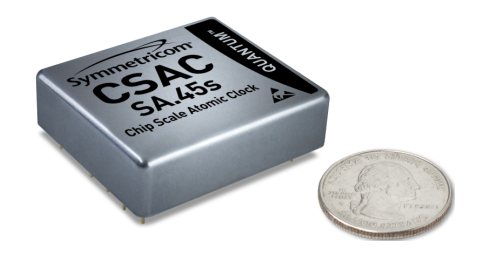
\includegraphics[width=0.7\columnwidth]{figures/microchip-csac}
        \caption{Microchip CSAC SA.45S atomic clock.}
        \label{fig:microchip-csac}
    \end{center}
\end{figure}

\subsection{Telecommunication analysis}

\subsubsection{Distance to Satellite at Horizon}

The distance to satellite at horizon (the maximum theoretical distance between the satellite and a ground station) can be calculated using \autoref{eq:horizon-distance}.

\begin{equation} \label{eq:horizon-distance}
d = \sqrt{2\cdot R_{e}\cdot h + h^{2}}
\end{equation}

Where:

\begin{itemize}
    \item $R_{e}$ = Earth radius = 6378 km
    \item $h$ = Satellite altitude = 550 km
    \item $d$ = Distance to sattellite at horizon
\end{itemize}

So, the distance to satellite at horizon is:

\begin{equation} \label{eq:horizon-distance-result}
d = \sqrt{2\cdot 6378\cdot 550 + 550^{2}} = \mathbf{2705\ km}
\end{equation}

\subsubsection{Free-Space Path Loss}

The free-space path loss ($FSPL$) can be calculated using \autoref{eq:fspl}.

\begin{equation} \label{eq:fspl}
FSPL = \left( \frac{4\pi d f}{c} \right)^{2}
\end{equation}

Where:

\begin{itemize}
    \item $d$ = Distance between the satellite and the ground station
    \item $f$ = Radio frequency
    \item $c$ = Speed of light
\end{itemize}

The FSPL value in decibels can be calculated with \autoref{eq:fsbl-db}.

\begin{equation} \label{eq:fsbl-db}
    \begin{split}
        FSPL^{dB} & = 20\log\left(\frac{4\pi}{c}\right) + 20\log\left(d\right) + 20\log\left(f\right) \\
                  & = 32,45 + 20\log\left(\frac{d}{1\ km}\right) + 20\log\left(\frac{f}{1\ MHz}\right) \\
    \end{split}
\end{equation}

The minimum distance between the satellite and a ground station is the satellite altitude, in this case: 600 km. The maximum distance is the distance at horizon, defined by \autoref{eq:horizon-distance-result}.

Considering the frequency of the beacon as 437 MHz, the minimum and maximum FSBL is:

\begin{equation}
    FSPL^{dB}_{min} = 32,45 + 20\log\left(\frac{550}{1\ km}\right) + 20\log\left(\frac{146}{1\ MHz}\right) = \mathbf{130,5\ dB}
\end{equation}

\begin{equation}
    FSPL^{dB}_{max} = 32,45 + 20\log\left(\frac{2705}{1\ km}\right) + 20\log\left(\frac{146}{1\ MHz}\right) = \mathbf{144,4\ dB}
\end{equation}

\begin{equation}
    \mathbf{130,5 \leq FSPL^{dB} \leq 144,4\ dB}
\end{equation}

\subsubsection{Power at Receiver}

The power of the signal at the receiver can be estimated using \autoref{eq:power-at-receiver}.

\begin{equation} \label{eq:power-at-receiver}
    P_{r} = P_{t} + G_{t} + G_{r} - L_{p} - L_{s}
\end{equation}

Where:

\begin{itemize}
    \item $P_{r}$ = Power at the receiver
    \item $P_{t}$ = Transmitter power
    \item $G_{t}$ = Antenna gain of the transmitter
    \item $G_{r}$ = Antenna gain of the receiver
    \item $L_{p}$ = FSPL (Free-Space Path Loss)
    \item $L_{s}$ = Other losses in the system
\end{itemize}

Considering the worst scenario with the maximum possible distance between the satellite and a ground station, the power at the receiver for the link is calculated below.

\begin{equation}
    P_{r} = 30 + 0 + 12 - 144,4 - 5 = -107,4\ dBm
\end{equation}

\begin{equation}
    \mathbf{P_{r} \geq -107,4\ dBm}
\end{equation}

\subsubsection{Signal-to-Noise-Ratio}

The Signal-to-Noise-Ratio (SNR) of a transmitted signal at the receiver can be expressed using \autoref{eq:snr}:

\begin{equation} \label{eq:snr}
    SNR = \frac{E_{b}}{N_{0}} = \frac{P_{t}G_{t}G_{r}}{kT_{s}RL_{p}}
\end{equation}

Where:

\begin{itemize}
    \item $P_{t}$ = Transmitter power
    \item $G_{t}$ = Antenna gain of the transmitter
    \item $G_{r}$ = Receiver gain
    \item $k$ = Boltzmann's constant ($\cong 1,3806 \times 10^{-23}\ J/K$)
    \item $T_{s}$ = System noise temperature
    \item $R$ = Data rate in bits per seconds (bps)
    \item $L_{p}$ = Free-Space Path Loss (FSPL)
\end{itemize}

The system noise temperature ($T_{s}$) can be defined using \autoref{eq:system-noise-temperature}.

\begin{equation} \label{eq:system-noise-temperature}
    T_{s} = T_{ant} + T_{r}
\end{equation}

with:

\begin{equation} \label{eq:noise-temperature-receiver}
    T_{r} = \frac{T_{0}}{L_{r}} (F - L_{r})
\end{equation}

and:

\begin{equation} \label{eq:noise-figure}
    F = 1 + \frac{T_{r}}{T_{0}}
\end{equation}

Combining Equations \ref{eq:system-noise-temperature}, \ref{eq:noise-temperature-receiver} and \ref{eq:noise-figure}:

\begin{equation} \label{eq:system-noise-temp-expanded}
    T_{s} = T_{ant} + \left( \frac{T_{0}(1 - L_{r})}{L_{r}} \right) + \left( \frac{T_{0} (F - 1)}{L_{r}} \right)
\end{equation}

Where:

\begin{itemize}
    \item $T_{ant}$ = Antenna noise temperature
    \item $T_{0}$ = Reference temperature (usually 290 K)
    \item $L_{r}$ = Line loss between the antenna and the receiver
    \item $F$ = Noise figure of the receiver
    \item $T_{r}$ = Noise temperature of the receiver
\end{itemize}

The SNR value in decibels can be calculated using the \autoref{eq:snr-db}:

\begin{equation} \label{eq:snr-db}
    \begin{split}
        SNR^{dB} & = 10\log_{10}\left( \frac{E_{b}}{N_{0}} \right) = 10\log_{10} \left( \frac{P_{t}G_{t}G_{r}}{kT_{s}RL_{p}} \right) \\
                 & = P_{t}^{dBm} - 30 + G_{t}^{dB} + G_{r}^{dB} - L_{p}^{dB} - 10\log k - 10\log T_{s} - 10\log R
    \end{split}
\end{equation}

Considering other losses in the system ($L_{s}$) (cable and connection losses as example), the \autoref{eq:snr-db} can be corrected as presented in \autoref{eq:snr-db-with-losses}.

\begin{equation} \label{eq:snr-db-with-losses}
    SNR^{dB} = P_{t}^{dBm} - 30 + G_{t}^{dB} + G_{r}^{dB} - L_{p}^{dB} - L_{s}^{dB} - 10\log k - 10\log T_{s} - 10\log R
\end{equation}

Using Equations \ref{eq:snr-db-with-losses} and \ref{eq:system-noise-temperature}, with:

\begin{itemize}
    \item $P_{t} = 30\ dBm$
    \item $G_{t} = 0\ dBi$
    \item $G_{r} = 12\ dBi$
    \item $L_{p} = 144,4\ dB$
    \item $L_{s} = 5\ dB$
    \item $R = 1200\ bps$
    \item $T_{0} = 290\ K$
    \item $T_{r} = 290\ K$
    \item $T_{ant} = 300\ K$
    \item $F = 2\ dB$
    \item $L_{r} = 0,89\ (0,5\ dB)$
\end{itemize}

\begin{equation}
    T_{s} = 300 + \left( \frac{290 (1 - 0,89)}{0,89} \right) + \left( \frac{290 (2 - 1)}{0,89} \right) = 661,7\ K
\end{equation}

\begin{equation}
    SNR^{dB} = 30 - 30 + 0 + 12 - 144,4 - 5 + 228,6 - 28,21 - 30,79 = 32,22\ dB
\end{equation}

\begin{equation}
\mathbf{SNR^{dB} \geq 32,22\ dB}
\end{equation}

\subsubsection{Link Margin}

From \cite{larson2005}, the minimum SNR value at the received considering a $10^{-5}$ bit error rate is:

\begin{itemize}
    \item Beacon: $SNR^{dB} \geq 9,6\ dB$
\end{itemize}

And considering the link margin as the SNR of the link minus the SNR threshold for a given bit error, the link margin of the radio links of the satellite are:

\begin{itemize}
    \item Beacon: $32,22 - 9,6 = \mathbf{22,62\ dB}$
\end{itemize}

\subsection{Power consumption analysis}

According to section 10.3 of \cite{larson2005}, the power budget of satellite can be determined through three steps:

\begin{enumerate}
    \item Prepare operating power budget
    \item Size the battery
    \item Estimate power degradation over mission life
\end{enumerate}

\subsubsection{Input Power}

A simulation of the energy input to the solar panels along some orbits can be seen in the \autoref{fig:sp_sim_power} graph. From this simulation, the following results were obtained:

\begin{itemize}
    \item Peak power $\cong$ 8759,5 mW
    \item Average (orbit) $\cong$ 2744,9 mW
    \item Average (sunlight) $\cong$ 4315,6 mW
    \item Orbit period $\cong$ 6018 sec
    \item Sun light period $\cong$ 3712 sec
    \item Eclipse period $\cong$ 2124 sec
\end{itemize}

\begin{figure}[!ht]
    \begin{center}
        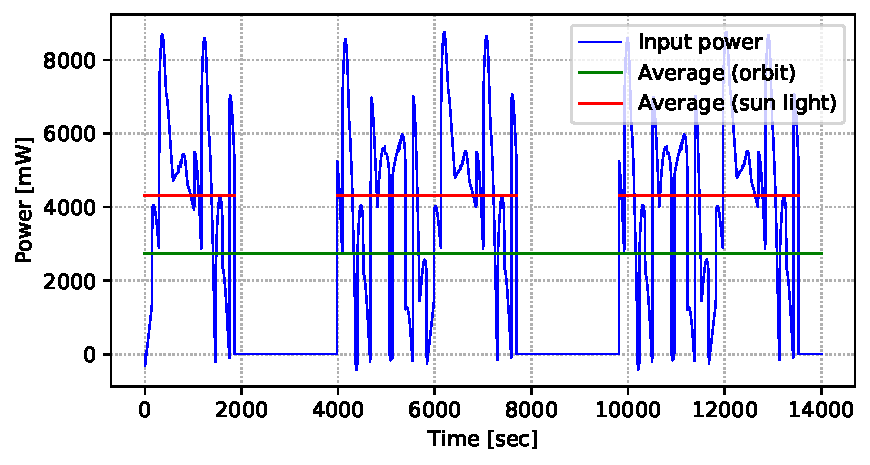
\includegraphics[width=\columnwidth]{curves/sp_sim_power}
        \caption{Silumated input power of the solar panels.}
        \label{fig:sp_sim_power}
    \end{center}
\end{figure}

\subsubsection{Operating Power Budget}

Typical operating voltages, and current and power ranges consumed by each satellite subsystem are presented in \autoref{tab:power-requirements}.

\begin{table}[!h]
    \centering
    \begin{tabular}{lccccc}
        \toprule[1.5pt]
        \multirow{2}{*}{\textbf{Module}} & \multirow{2}{*}{\textbf{Voltage [V]}}    & \multicolumn{2}{c}{\textbf{Current [mA]}} & \multicolumn{2}{c}{\textbf{Power [mW]}} \\
                                         &                                          & \textbf{Min.} & \textbf{Max.}             & \textbf{Min.} & \textbf{Max.} \\
        \midrule
        OBDH                & 3,3   & 35    & 200   & 115   & 660 \\
        TTC ($\mu$C)        & 3,3   & 40    & 40    & 132   & 132 \\
        TTC (radio module)  & 5     & 10    & 650   & 33    & 3250 \\
        EPS (digital part)  & 7,4   & 50    & 260   & 165   & 858 \\
        EPS (heater)        & 7,4   & 675   & 675   & 5000  & 5000 \\
        Antenna module      & 3,3   & 60    & 550   & 200   & 1800 \\
        Payload EDC         & 5     & 250   & 250   & 1250  & 1250 \\
        Payload-X           & 5     & TBD   & TBD   & TBD   & TBD \\
        Payload Harsh       & 3,3   & TBD   & TBD   & TBD   & TBD \\
        \bottomrule[1.5pt]
    \end{tabular}
    \caption{Power requirements of the subsystems and payloads of the satellite.}
    \label{tab:power-requirements}
\end{table}

Using the information presented in \autoref{tab:power-requirements}, and the activation periods defined for each module (the duty cycle), we arrive at the average satellite consumption present in \autoref{tab:power-consumption}.

\begin{table}[!h]
    \centering
    \begin{tabular}{lccccc}
        \toprule[1.5pt]
        \textbf{Module} & \textbf{Duty Cycle [\%]}    & \textbf{Power [mW]} \\
        \midrule
        OBDH                    & 100   & 115 \\
        TTC (radio 1 RX)        & 95    & 65 \\
        TTC (radio 1 TX)        & 5     & 3250 \\
        TTC (radio 2 RX)        & 95    & 65 \\
        TTC (radio 2 TX)        & 5     & 3250 \\
        EPS                     & 100   & 320 \\
        BAT (idle)              & 90    & 0 \\
        BAT (heater full)       & 10    & 5000 \\
        Antenna (deployment)    & 0     & 1800 \\
        Antenna (deployed)      & 100   & 35 \\
        Payload EDC             & 100   & 1250 \\
        Payload Harsh           & 0     & 330 \\
        Payload-X               & 0     & 1000 \\
        \cmidrule{2-3}
        Satellite               & \multicolumn{2}{c}{$\cong$ 2668} \\
        \bottomrule[1.5pt]
    \end{tabular}
    \caption{Power consumption of the subsystems and payloads of the satellite.}
    \label{tab:power-consumption}
\end{table}

The duty cycles of \autoref{tab:power-consumption} were defined according to the following assumptions:

\begin{itemize}
    \item One of the EDC payload is always off (cold redundancy).
    \item The Payload-X and the Harsh payload are turned on just during limited periods and only with telecommands.
\end{itemize}

As can be seen from \autoref{fig:sp_sim_power} and \autoref{tab:power-consumption}, there is a slight positive margin of \textbf{76,9 mW} in the power budget.

\subsection{Orbit analysis}

To define the orbit parameters and simulate the behaviour of the satellite during its operation, the GMAT software was used \cite{gmat}. The orbit parameters was based on the FloripaSat-I TLE, but with a lower altitude. These parameters can be seen in \autoref{tab:orbit-parameters}.

\begin{table}[!h]
    \centering
    \begin{tabular}{lcc}
        \toprule[1.5pt]
        \textbf{Parameters} & \textbf{Value} & \textbf{Unit} \\
        \midrule
        Altitude                & 550           & km \\
        Eccentricity            & 0,0015051     & $^{\circ}$ \\
        Inclination             & 97,9750       & $^{\circ}$ \\
        RAAN                    & 85,5100       & $^{\circ}$ \\
        Arg. of Perigee (AOP)   & 194,87        & $^{\circ}$ \\
        TA                      & 99,8877       & $^{\circ}$ \\
        \bottomrule[1.5pt]
    \end{tabular}
    \caption{Initial orbit parameters (adapted from FloripaSat-I).}
    \label{tab:orbit-parameters}
\end{table}

The parameters of the simulation on GMAT was based on \cite{marino2016} and can be seen below:

\begin{itemize}
    \item Force model for gravitational field: ``\textit{Earth Gravitational Model 1996 (EGM96)}''
    \item Propagator: ``\textit{PrinceDorman78}''
    \item Drag coefficient: 2,2
    \item Drag atmosphere model: ``\textit{Mass Spectrometry and Incoherent Scatter (MSISE90)}''
    \item Epoch: 01 Jan 2022 11:59:28.000
\end{itemize}

The \autoref{fig:fsat2-gmat} shows the 3D representation of the FloripaSat-2 orbit simulation, \autoref{fig:fsat2-gmat-groundtrack} shows the ground track of the first day of operation.

\begin{figure}[!ht]
    \begin{center}
        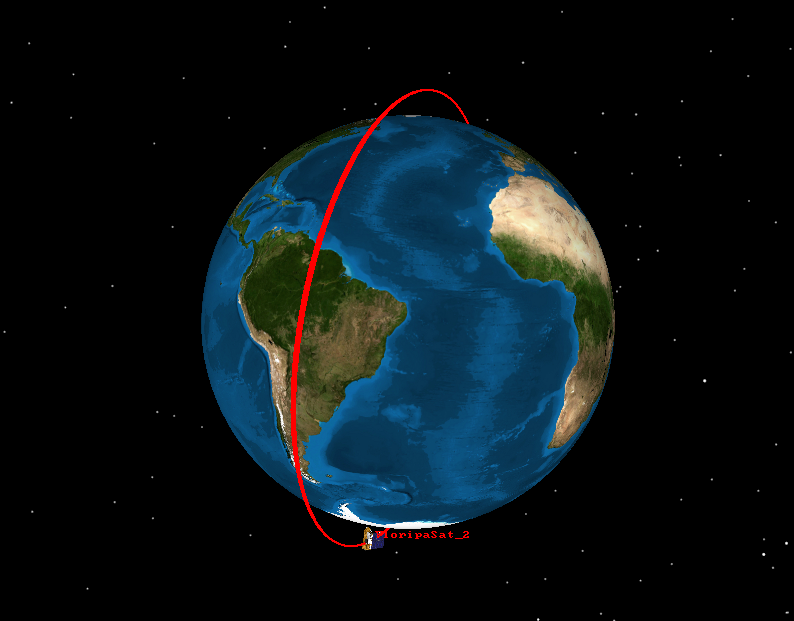
\includegraphics[width=0.6\columnwidth]{figures/fsat2-gmat.png}
        \caption{FloripaSat-2 orbit simulation on GMAT.}
        \label{fig:fsat2-gmat}
    \end{center}
\end{figure}

\begin{figure}[!ht]
    \begin{center}
        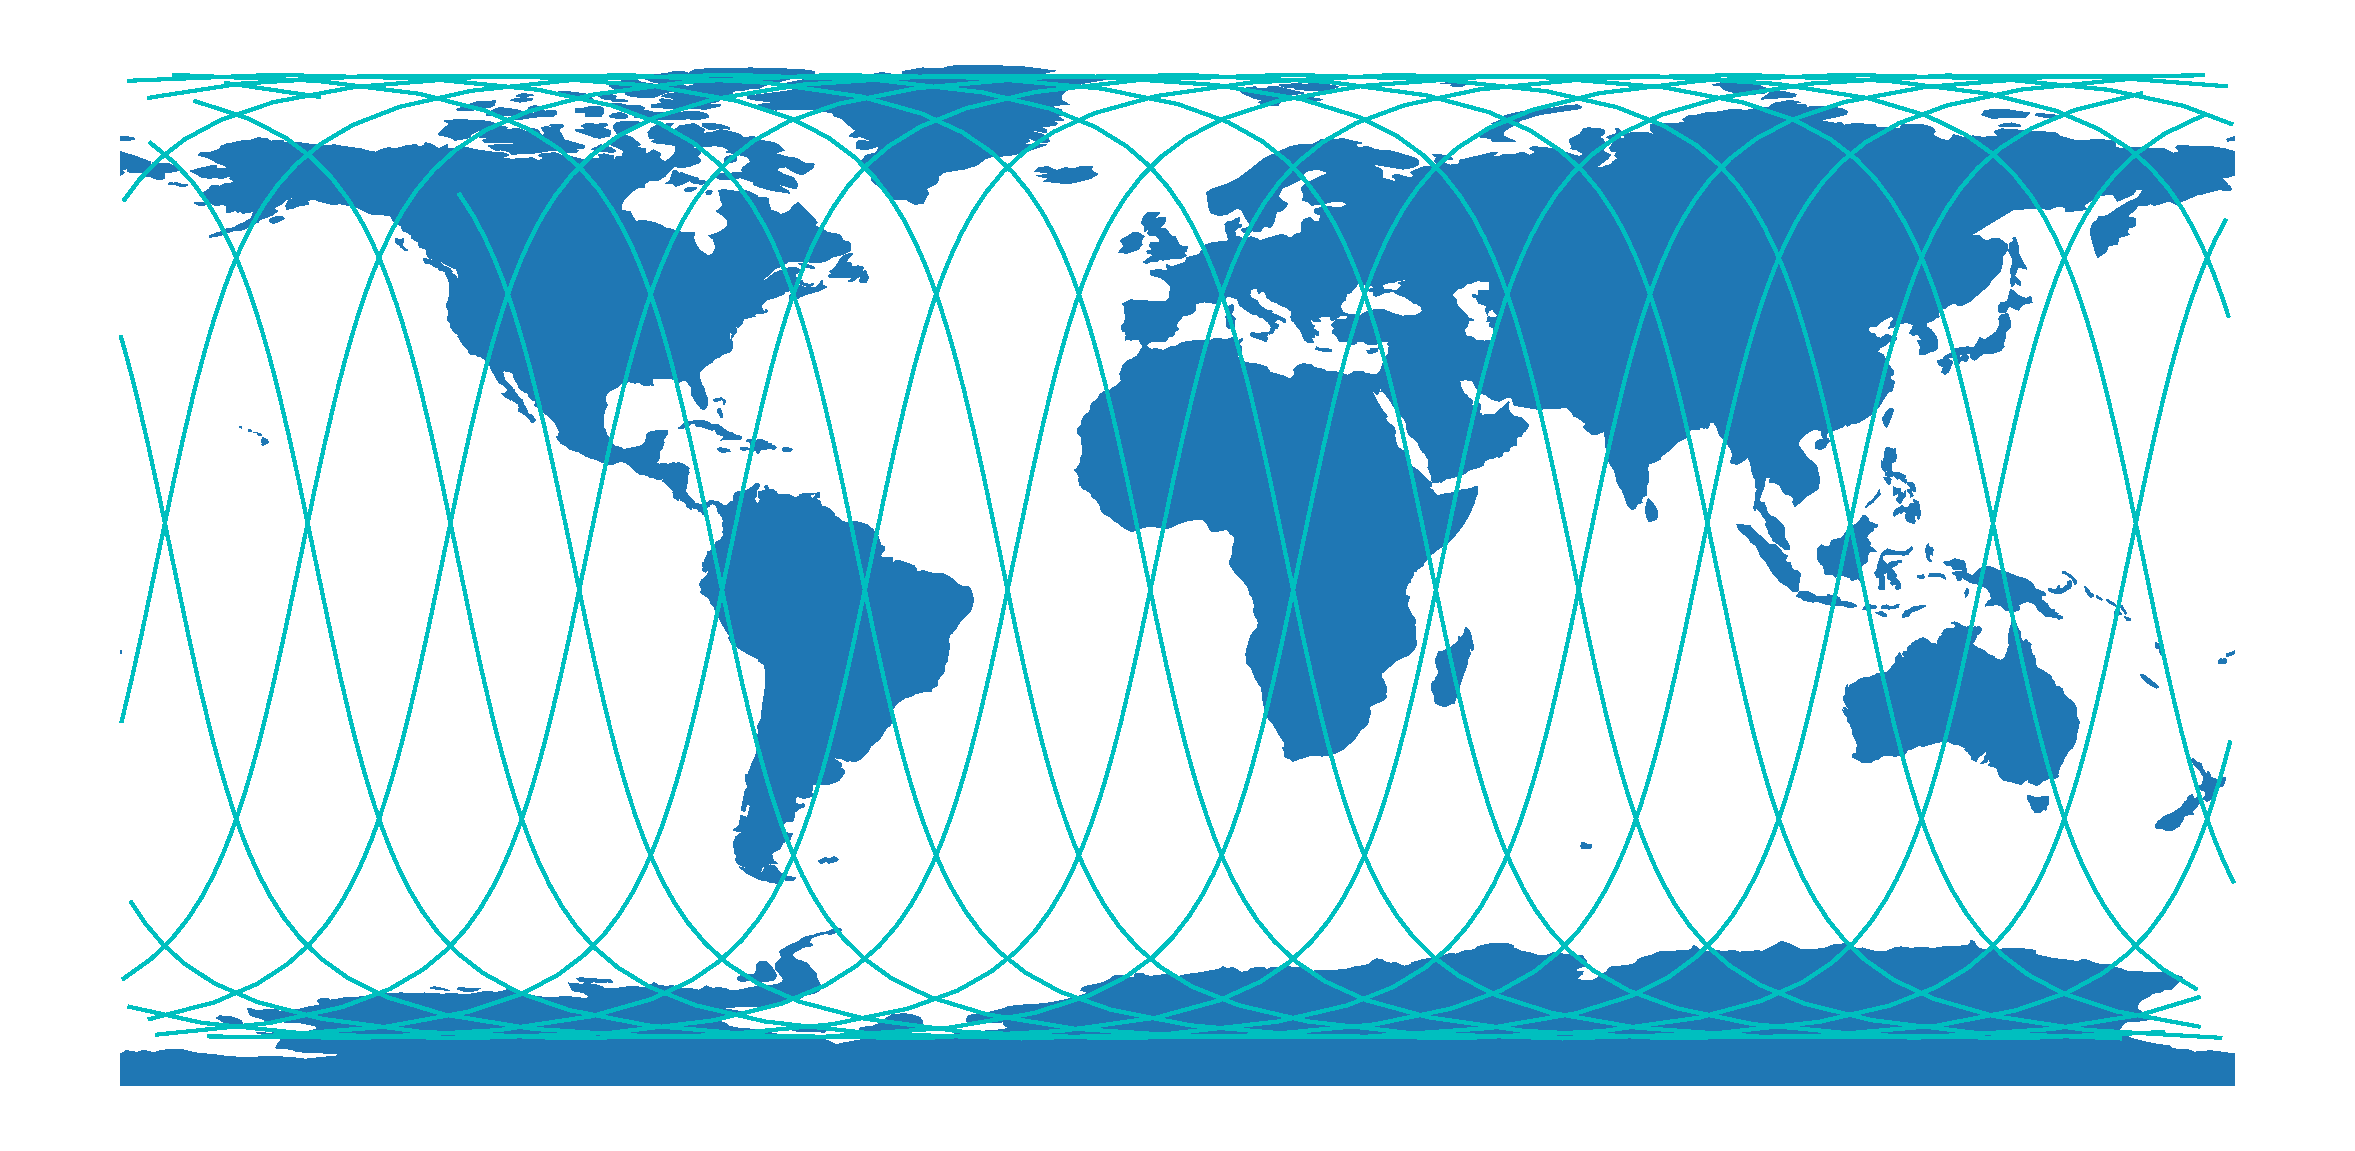
\includegraphics[width=\columnwidth]{figures/fsat2-gmat-groundtrack.pdf}
        \caption{FloripaSat-2 simulated groundtrack.}
        \label{fig:fsat2-gmat-groundtrack}
    \end{center}
\end{figure}

The next sections present some analysis based on the results obtained on the simulations executed on GMAT.

The source files of the GMAT simulation are available in \cite{fsat2-mechanical}.

\subsubsection{Lifetime Analysis}

Considering the same parameters of FloripaSat-I, but with an initial altitude of 550 km, the simulations on GMAT showed that the satellite decays approximately in 2000 days ($\cong$ 5 years), as can be seen in \autoref{fig:lifetime-analysis}.

\begin{figure}[!ht]
    \begin{center}
        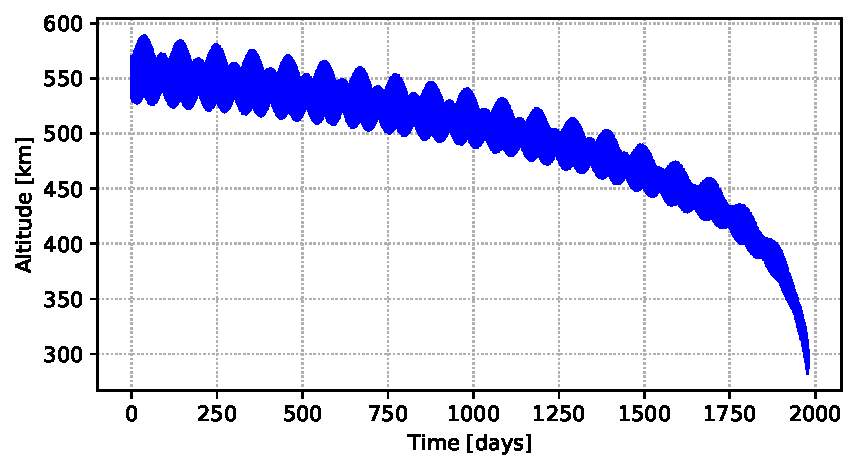
\includegraphics[width=\columnwidth]{curves/lifetime.pdf}
        \caption{Lifetime analysis on GMAT.}
        \label{fig:lifetime-analysis}
    \end{center}
\end{figure}
